\begin{figure}[!htbp]
\centering
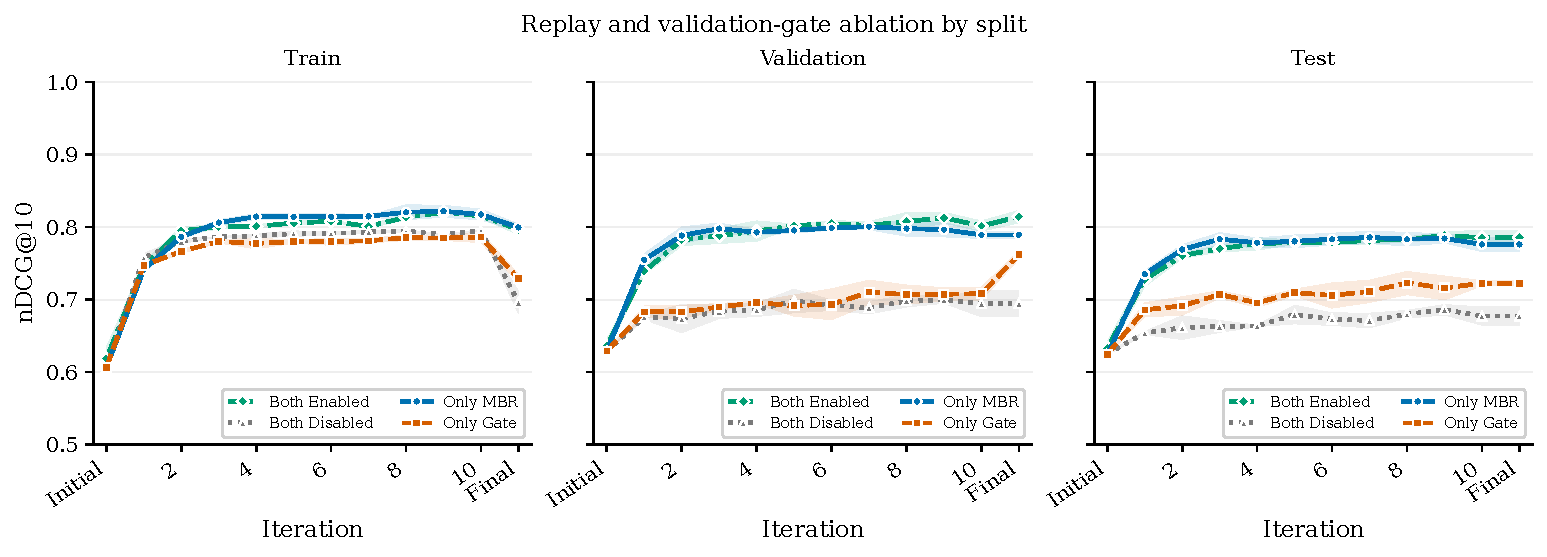
\includegraphics[width=\linewidth]{figs/mbr_replay_validation_std_all_splits/preview.pdf}
\caption{Replay and validation-gate ablation across train, validation, and test splits. Analysis-only (non-reportable or unknown source provenance). Task-weighted source Dataset=Average rows for train, validation, and test (task-weighted over instances within each split/evaluation); train uses prequential scores, validation uses ledger-accepted-candidate scores, and test uses accepted-candidate scores. Initial and final are snapshot checkpoints (plotted at 0 and 11); iterations 1–10 use their source evaluation stage. Lines show nDCG@10 means; shaded bands show mean ± one population standard deviation from the supplied variance (not confidence intervals); three observed runs per checkpoint.}
\label{fig:mbr_replay_validation_std_all_splits}
\end{figure}
